\subsection{Debug Window Size}
\label{sec:timewindowPerformance}

To understand the size of the debug-window and it's dependence on resources, we did some experiments on real-world applications, by introducing a delay while duplicating the network input.
This gave us some real-world idea of buffer overflow and it's relationship to the buffer size and input workload.
Since it was difficult to observe systematic behavior in a live system to understand the decay rate of the debug-window, we also did some simulation experiments, to see how soon the buffer would overflow for different input criteria.

\xxx{We did some experiments, and also simulations because... The setup was... The buffer size was...}
\yyy{added the reason, as a small intro}
\begin{table}[ht]
	\centering
\setlength{\tabcolsep}{2pt}
	\begin{tabular}{c r r r }
		\toprule
		{\bf Input Rate} & \textbf{Debug Window} & \textbf{Pipe Size} & \textbf{Slowdown} \\ \midrule
		530 bps, 27 rq/s                                            & $\infinity$                                                                                     & 4096                                                                            & 1.8x                                                                             \\ %\hline
		530 bps, 27 rq/s                                            & 8 sec                                                                              & 4096                                                                            & 3x                                                                               \\ %\hline
		530 bps, 27 rq/s                                            & 72 sec                                                                             & 16384                                                                           & 3x                                                                               \\ %\hline
		Pois., $\lambda$ = 17 rq/s                                        & 16 sec                                                                             & 4096                                                                            & 8x                                                                               \\ %\hline
Pois.,		$\lambda$ = 17 rq/s                                        & 18 sec                                                                             & 4096                                                                            & 5x                                                                               \\ %\hline
		Pois.,$\lambda$ = 17 rq/s                                        & $\infinity$                                                                                     & 65536                                                                           & 3.2x                                                                             \\ %\hline
		Pois.,$\lambda$ = 17 rq/s                                        & 376 sec                                                                            & 16384                                                                           & 3.2x                                                                             \\ %\hline
		\bottomrule
	\end{tabular}
	%\captionsetup{justification=centering}
	\caption{Approximate debug window sizes for a MySQL request workload}
	\label{table:timewindow}
\end{table}

\noindent
\textbf{Experimental Results:} We call the time taken to reach a buffer overflow the ``debug-window''.
As explained earlier, the size of this debug-window depends on the overhead of the ``instrumentation'', the incoming workload distribution, and the size of the buffer.
To evaluate the approximate size of the debug-window, we sent requests to both a production and debug MySQL container via our network duplicator.
Each workload ran for about 7 minutes (10,000 ``select * from table'' queries), with varying request workloads.
We also profiled the server, and found that is able to process a max of 27 req/s\footnote{Not the same as bandwidth, 27 req/s is the maximum rate of sequential requests MySQL server is able to handle for a user session} in a single user connect session. 
For each of our experiments, we vary the buffer sizes to get an idea of debug-window. 
Additionally, we generated a slowdown by first modeling the time taken by MySQL to process requests (27 req/s or 17req/s), and then putting an approximate sleep in the request handler.

Initially, we created a connection and sent requests at the maximum request rate the server was able to handle (27 req/s).
We found that for overheads up-to 1.8x (approx) we experienced no buffer overflows.
For higher overheads the debug window rapidly decreased, primarily dependent on buffer-size, request size, and slowdown.

Next, we mimic user behavior, to generate a realistic workload.
We send packets using a Poisson process with an average request rate of 17 requests per second to our proxy. 
This varies the inter-request arrival time, and let's the cloned debug-container catch up with the production container during idle time-periods in between request bursts.
We observed, that compared to earlier experiments, there was more slack in the system. 
This meant that our system was able to tolerate a much higher overhead (3.2x) with no buffer overflows.


\begin{figure}[ht]
	%{0.45\textwidth}
	\centering
	\resizebox{.85\linewidth}{!}{
		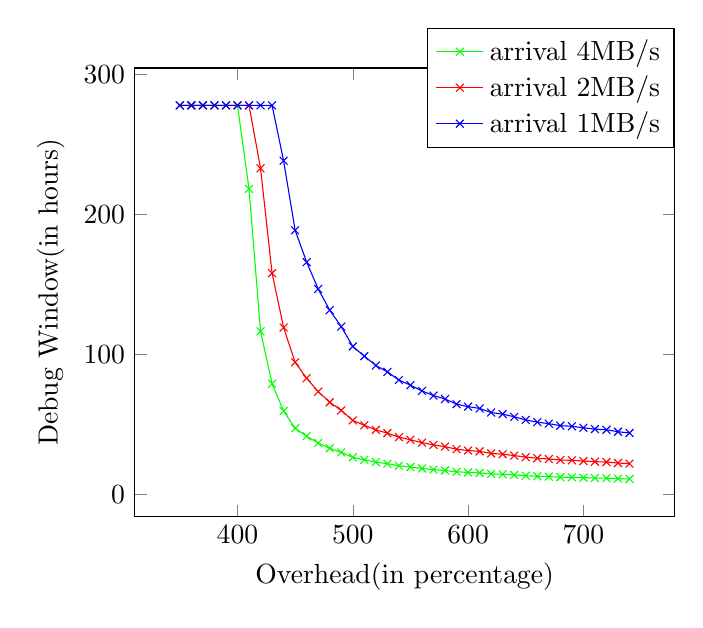
\begin{tikzpicture}
		\begin{axis}[
		%xmode=log,
		legend style={at={(1,1.09)},anchor=north east,legend columns=1},
		xlabel=Overhead(in percentage),
		ylabel=Debug Window(in hours)]
		\addplot[color=green,mark=x] coordinates {
			(350,277.7778028)
			(360,277.7778306)
			(370,277.7777806)
			(380,277.7777806)
			(390,277.777875)
			(400,277.7777972)
			(410,218.0984611)
			(420,116.3991028)
			(430,78.9657)
			(440,59.55381111)
			(450,47.147775)
			(460,41.446375)
			(470,36.65794167)
			(480,32.87560278)
			(490,29.95016111)
			(500,26.40129444)
			(510,24.66028333)
			(520,23.00362222)
			(530,21.85588056)
			(540,20.40405)
			(550,19.48659444)
			(560,18.45943611)
			(570,17.63081111)
			(580,17.01690833)
			(590,16.09901389)
			(600,15.65028056)
			(610,15.33356944)
			(620,14.601075)
			(630,14.32908611)
			(640,13.83495833)
			(650,13.29390556)
			(660,12.88229722)
			(670,12.61861944)
			(680,12.25779722)
			(690,12.14353889)
			(700,11.8762)
			(710,11.64855)
			(720,11.52348611)
			(730,11.17581111)
			(740,10.95483889)
		};
		\addlegendentry{arrival 4MB/s}
		\addplot[color=red,mark=x] coordinates {
			(350,277.7778361)
			(360,277.7777917)
			(370,277.7778389)
			(380,277.7778222)
			(390,277.7777806)
			(400,277.7778056)
			(410,277.7777778)
			(420,232.7982083)
			(430,157.9314)
			(440,119.1076194)
			(450,94.29555)
			(460,82.89275)
			(470,73.31588611)
			(480,65.75120278)
			(490,59.90032222)
			(500,52.80259167)
			(510,49.32056944)
			(520,46.00724722)
			(530,43.71176389)
			(540,40.80809722)
			(550,38.97319167)
			(560,36.91887222)
			(570,35.26162222)
			(580,34.03381667)
			(590,32.19803056)
			(600,31.30056389)
			(610,30.66714167)
			(620,29.20215)
			(630,28.65817222)
			(640,27.66991667)
			(650,26.58781389)
			(660,25.76459444)
			(670,25.23723611)
			(680,24.51559722)
			(690,24.28707778)
			(700,23.75239722)
			(710,23.2971)
			(720,23.046975)
			(730,22.35162222)
			(740,21.909675)
		};
		\addlegendentry{arrival 2MB/s}				
		\addplot[color=blue,mark=x] coordinates {
			(350,277.7778694)
			(360,277.7777944)
			(370,277.7779611)
			(380,277.7778389)
			(390,277.7777889)
			(400,277.7779139)
			(410,277.7778056)
			(420,277.7778167)
			(430,277.777875)
			(440,238.2152389)
			(450,188.5911)
			(460,165.7855028)
			(470,146.6317694)
			(480,131.5024056)
			(490,119.8006444)
			(500,105.6051806)
			(510,98.64113611)
			(520,92.01449444)
			(530,87.42352778)
			(540,81.61619722)
			(550,77.94638056)
			(560,73.83774444)
			(570,70.52324444)
			(580,68.06763333)
			(590,64.39605833)
			(600,62.60112778)
			(610,61.33428056)
			(620,58.40430278)
			(630,57.31634722)
			(640,55.33983056)
			(650,53.175625)
			(660,51.52919167)
			(670,50.474475)
			(680,49.03119167)
			(690,48.57415278)
			(700,47.50479722)
			(710,46.59420278)
			(720,46.09394722)
			(730,44.70324722)
			(740,43.81935)
		};
		\addlegendentry{arrival 1MB/s}				
		\end{axis}
		\end{tikzpicture}
	 }
	%\captionsetup{justification=centering}
	\caption{Simulation results for debug-window size. Each series has a constant arrival rate, and the buffer is kept at 64GB.}
	\label{fig:debugSim}
\end{figure}

\noindent
\textbf{Simulation Results:} 
In our next set of experiments, we simulate packet arrival and service processing for a buffered queue in SOA applications. 
We use a discrete event simulation based on an M\/M\/1 queue, which is a  classic queuing model based on Kendall's notation~\cite{kendall1953}, and is often used to model SOA applications with a single buffer based queue.
Essentially, we are sending and processing requests based on a Poisson distribution with a finite buffer capacity.
In our simulations (see Figure~\ref{fig:debugSim}), we kept a constant buffer size of 64GB, and iteratively increased the overhead of instrumentation, thereby decreasing the service processing time.
Each series (set of experiments), starts with an arrival rate approximately 5 times less than the service processing time. 
This means that at 400\% overhead, the system would be running at full capacity (for stable systems SOA applications generally operate at much less than system capacity).
Each simulation instance was run for 1000000 seconds or 277.7 hours.
We gradually increased the instrumentation by 10\% each time, and observed the \textit{hitting-time} of the buffer (time it takes for the buffer to overflow for the first time).
As shown there is no buffer overflow in any of the simulations until the overhead reaches around 420-470\%, beyond this the debug-window decreases exponentially.
Since beyond 400\% overhead, the system is over-capacity, the queue will start filling up fairly quickly. 
This clarifies the behavior we observed in our experiments, where for lower overheads (1.8-3.2x) we did not observe any overflow, but beyond a certain point, we observed that the buffer would overflow fairly quickly.
Also as shown in the system, since the buffer size is significantly larger than the packet arrival rate, it takes some time for the buffer to overflow (several hours).
We believe that while most systems will run significantly under capacity, large buffer sizes can ensure that our debug-container may be able to handle short bursts in the workload.
However, a system running continuously at capacity is unlikely to tolerate significant instrumentation overhead.\\ \\
%For more details regarding queuing theory models and our detailed simulations, please have a look at our extended tech-report tech-report~\cite{parikshanQueue}.

\xxx{Good to show here a list of example dynamic analyses that would fit within the window. So, say, our GOAL is to be able to support running dynamic analyses X, Y, Z. X, Y, and Z usually have an overhead of 1.5X, which is WAY too slow to use in production. BUT can we use them in our debug environments? YES!}


\begin{tcolorbox}[breakable, enhanced]
		To answer \textbf{RQ2}, we found that the debug-container can stay in a stable state without any buffer overflows as long as the instrumentation does not cause the service times to become less than the request arrival rate. Furthermore, a large buffer will allow handling of short bursts in the workload until the system returns back to a stable state. The debug-window can allow for a significant slowdown, which means that many existing dynamic analysis techniques~\cite{dpor,valgrind}, as well as most fine-grained tracing~\cite{fay,failuresketching} can be applied on the debug-container without leading to an incorrect state.
\end{tcolorbox}



\iffalse
\begin{table}[ht]
\begin{centering}
\begin{tabular}{|c|c|c|c|}
\hline
\begin{tabular}[c]{@{}c@{}}\textbf{Input} \\ \textbf{Rate}\end{tabular} & \begin{tabular}[c]{@{}c@{}}\textbf{Debug}\\ \textbf{Window}\end{tabular} & \begin{tabular}[c]{@{}c@{}}\textbf{Pipe}\\ \textbf{Size}\end{tabular} & \begin{tabular}[c]{@{}c@{}}\textbf{Slow-}\\ \textbf{down}\end{tabular}\\ \hline
530 bps, 27 rq/s                                      & $\infinity$                                                    & 4096                                                & 1.8x                      \\ \hline
530 bps, 27 rq/s                                      & 8 sec                                                  & 4096                                                & 3x                        \\ \hline
530 bps, 27 rq/s                                      & 72 sec                                                 & 16384                                               & 3x                        \\ \hline
Poisson, $\lambda$ = 17 rq/s                               & 16 sec                                                 & 4096                                                & 8x                        \\ \hline
Poisson, $\lambda$ = 17 rq/s                               & 18 sec                                                 & 4096                                                & 5x                      \\ \hline
Poisson, $\lambda$ = 17 rq/s                               & $\infinity$                                                    & 65536                                               & 3.2x \\ \hline
Poisson, $\lambda$ = 17 rq/s                               & 376 sec                                                & 16384                                               & 3.2x \\ \hline
\end{tabular}
\captionsetup{justification=centering}
\caption{Approximate debug window sizes for a MySQL request workload}
\label{table:timewindow}
\end{centering}
\end{table}
\fi